\hsection{Creating a new Database}%
\begin{figure}%
\centering%
%
\subfloat[][%
As in \cref{fig:psqlNewUser1starting}, we open a console via \ubuntuTerminal\ under \ubuntu\ \linux\ or by \windowsTerminal\ under \microsoftWindows. %
We connect the \psql\ \pgls{client} to the \postgresql\ \pgls{server} listening at the default port on our current computer~(\localhost) and tell it to log in as user \textil{postgresql} with the password~\textil{XXX} and hit~\keys{\enter}. %
Notice:~We can also put the \pgls{URI} in quotes, which is good if the password contains strange characters.%
\label{fig:createDB01start}%
]{\parbox[t]{0.99\linewidth}{\centering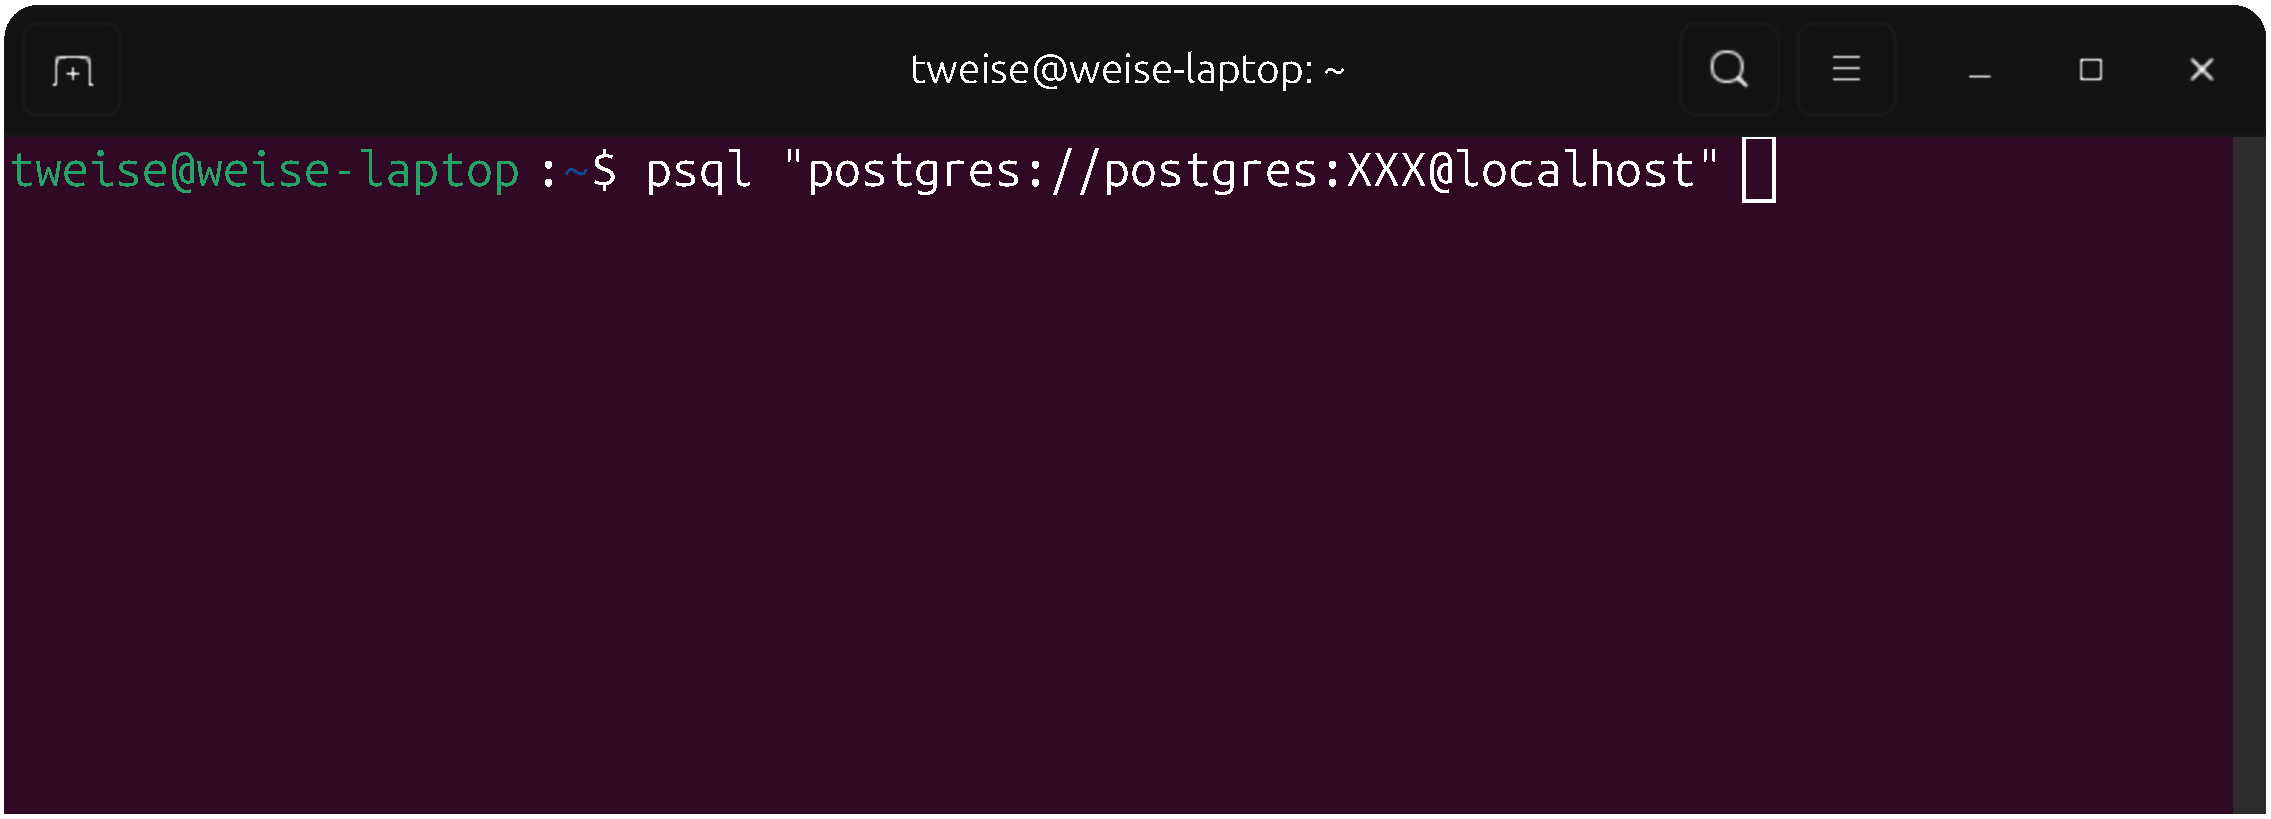
\includegraphics[width=0.67\linewidth]{\currentDir/createDB01start}}}%
%
\floatRowSep%
%
\subfloat[][%
As in \cref{fig:psqlNewUser2psqlOpen}, the \psql\ session is now open.%
\label{fig:createDB02started}%
]{\parbox[t]{0.99\linewidth}{\centering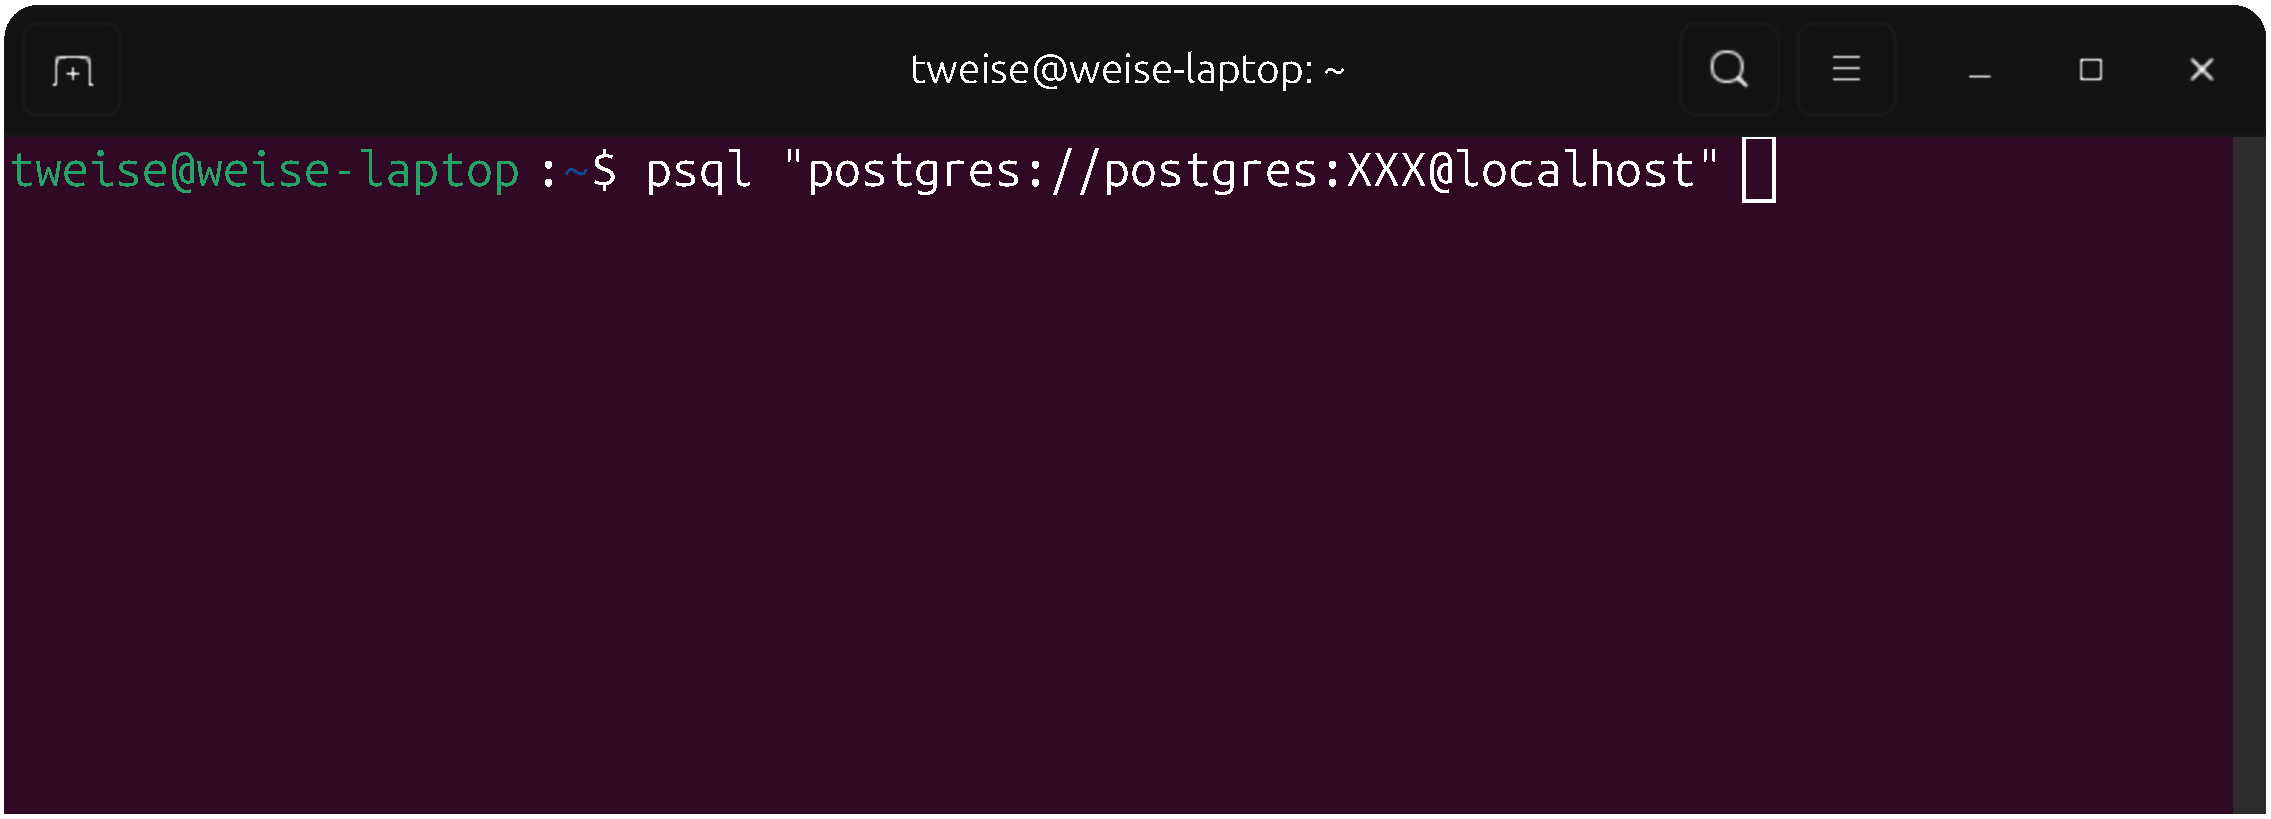
\includegraphics[width=0.67\linewidth]{\currentDir/createDB01start}}}%
%
\floatRowSep%
%
\subfloat[][%
We type in the command \sqlil{CREATE DATABASE factory OWNER boss}\sqlIdx{CREATE!DATABASE} which will create the \db\ \sqlil{facory}. %
The parameter \sqlil{OWNER boss}\sqlIdx{OWNER} sets the new user \sqlil{boss} to be the owner of this \db.%
\label{fig:createDB03createDatabase}%
]{\parbox[t]{0.99\linewidth}{\centering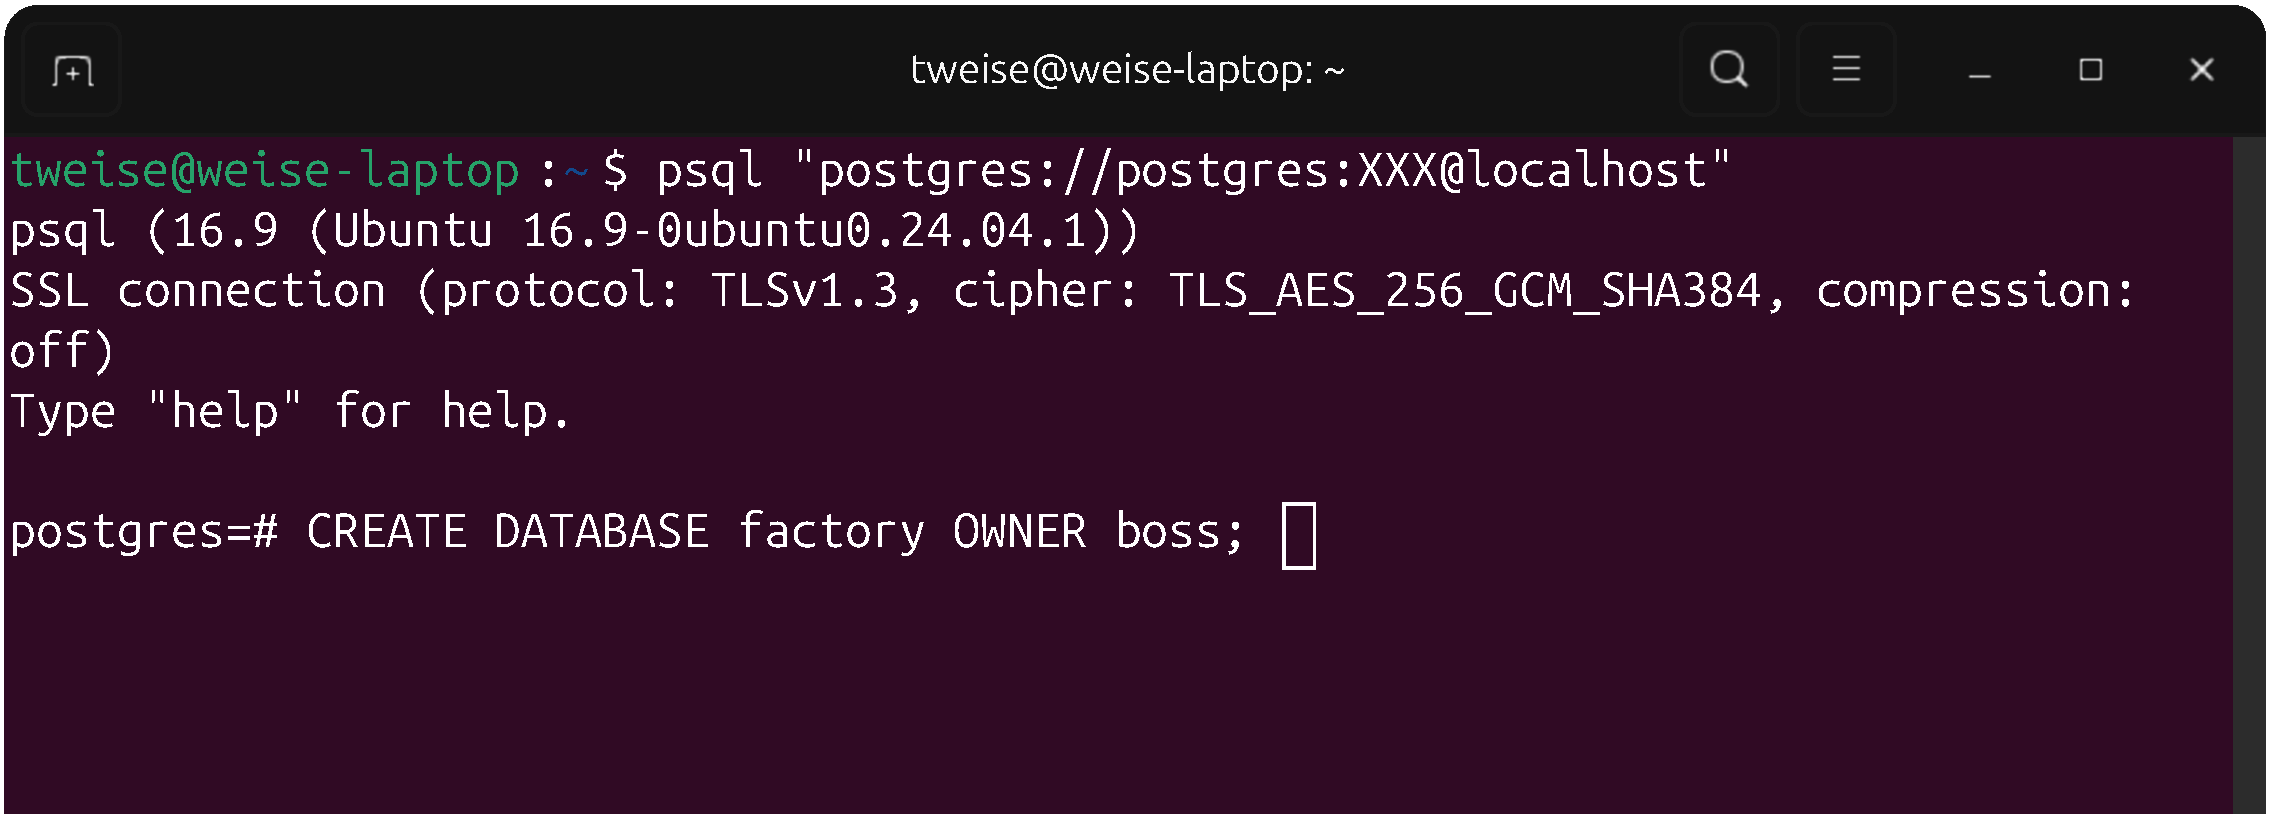
\includegraphics[width=0.67\linewidth]{\currentDir/createDB03createDatabase}}}%
%
\floatRowSep%
%
\subfloat[][%
To indicate success, \psql\ prints the command back to us\sqlIdx{CREATE!DATABASE}.%
\label{fig:createDB04dbCreated}%
]{\parbox[t]{0.99\linewidth}{\centering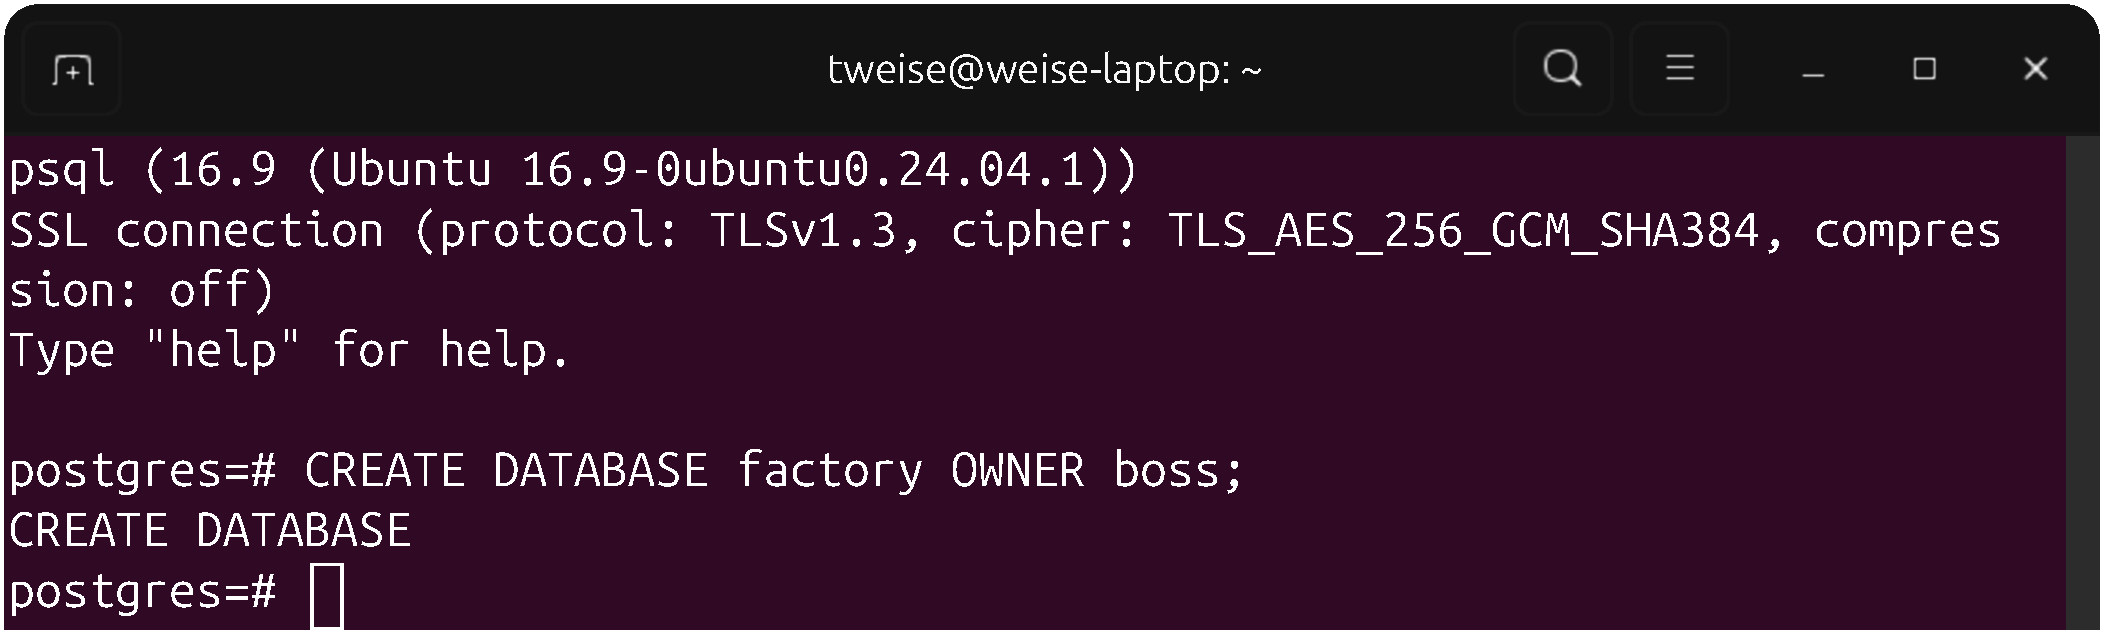
\includegraphics[width=0.67\linewidth]{\currentDir/createDB04dbCreated}}}%
%
\caption{Creating a new \db, adding a comment to it, and checking whether it really was created, all via \psql.}%
\end{figure}%
%
\begin{figure}%
\centering%
\ContinuedFloat%
%
\subfloat[][%
We can add comments to many of the elements that we create. %
Comments are good for documenting the meaning and reasons of the \db\ elements. %
Therefore, by using the \sqlil{COMMENT ON ... IS}\sqlIdx{COMMENT ON}\sqlIdx{IS} command, we add some documentation to our new \db.%
\label{fig:createDB05comment}%
]{\parbox[t]{0.99\linewidth}{\centering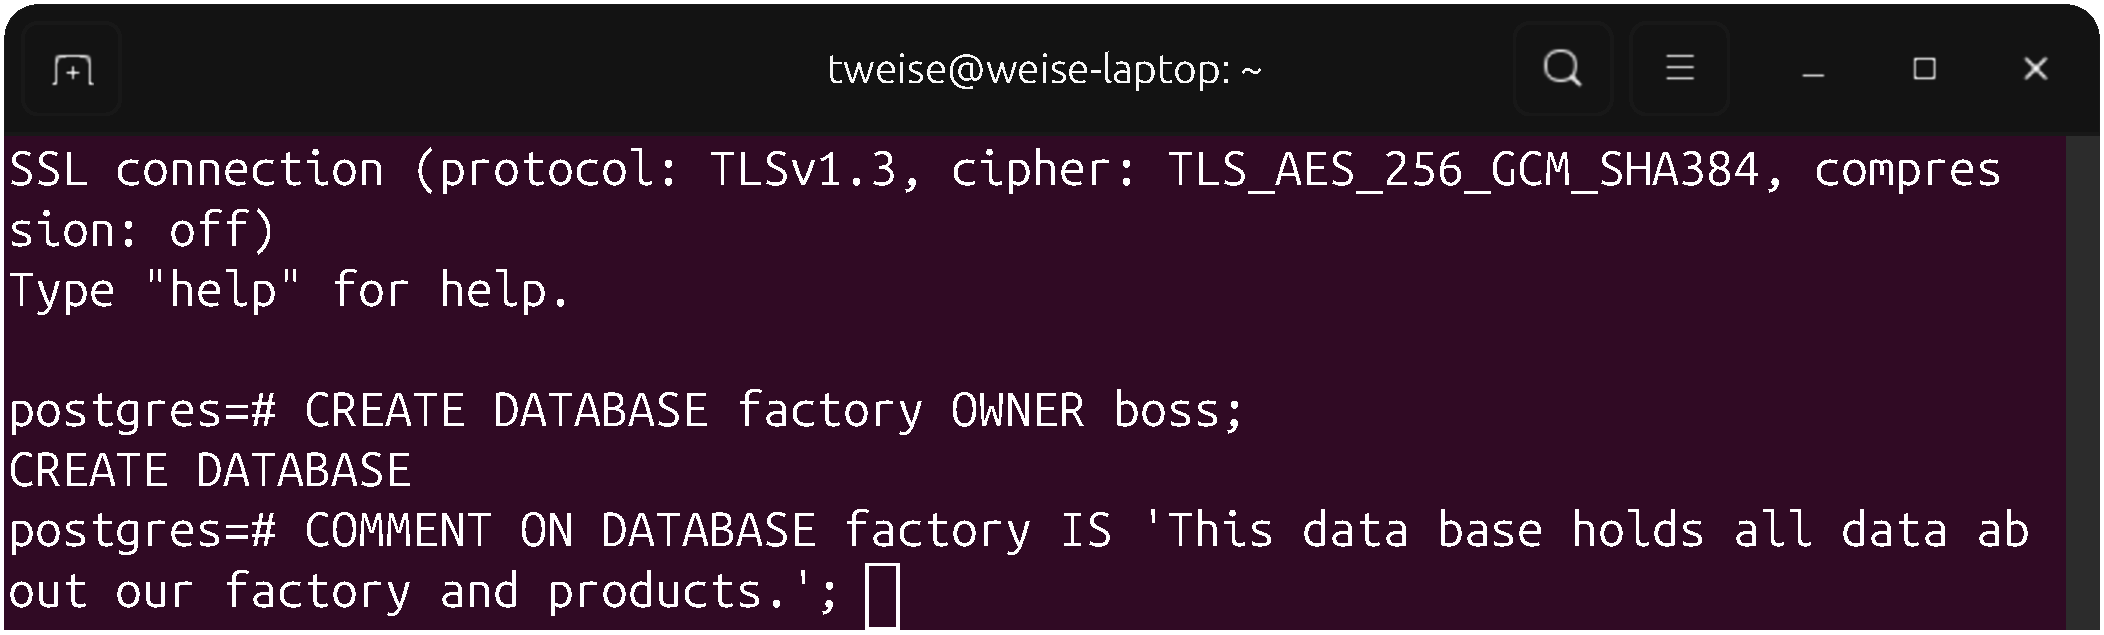
\includegraphics[width=0.67\linewidth]{\currentDir/createDB05comment}}}%
%
\floatRowSep%
%
\subfloat[][%
To indicate success, \psql\ prints the command back to us.%
\label{fig:createDB06commented}%
]{\parbox[t]{0.99\linewidth}{\centering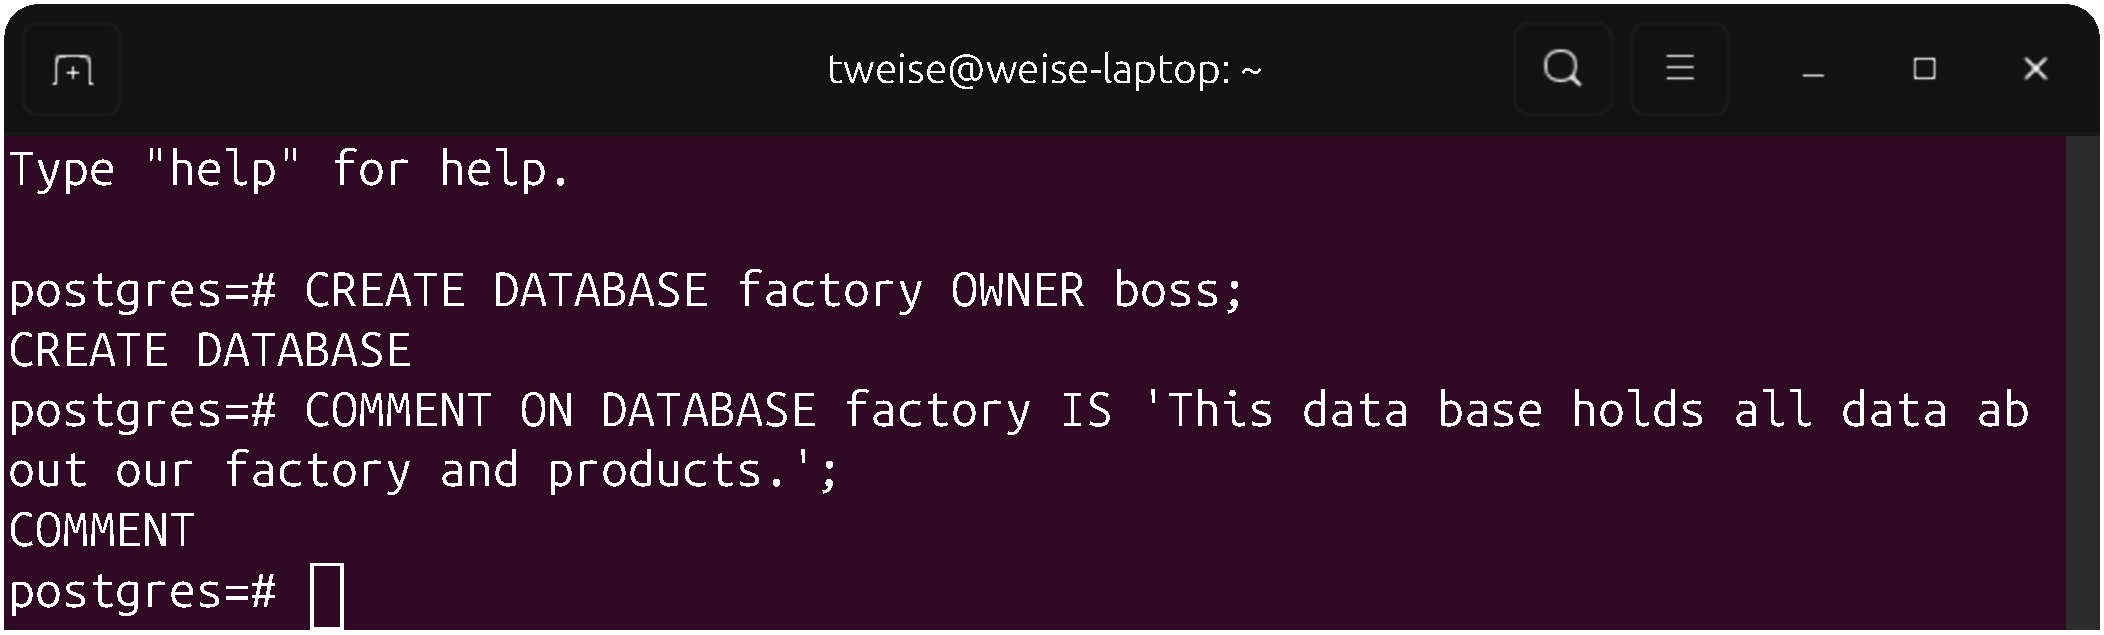
\includegraphics[width=0.67\linewidth]{\currentDir/createDB06commented}}}%
%
\floatRowSep%
%
\subfloat[][%
We now want to see the list of all \pglspl{db} in our \dbms. %
We therefore type the command \sqlil{SELECT datname FROM pg_database;}\sqlIdx{SELECT{\idxdots}FROM}. %
\sqlil{pg_database}\sqlIdx{pg\_databases} is a system table holding all \pglspl{db}, and its column \sqlilIdx{datname} contains their names.%
\label{fig:createDB07selectDatname}%
]{\parbox[t]{0.99\linewidth}{\centering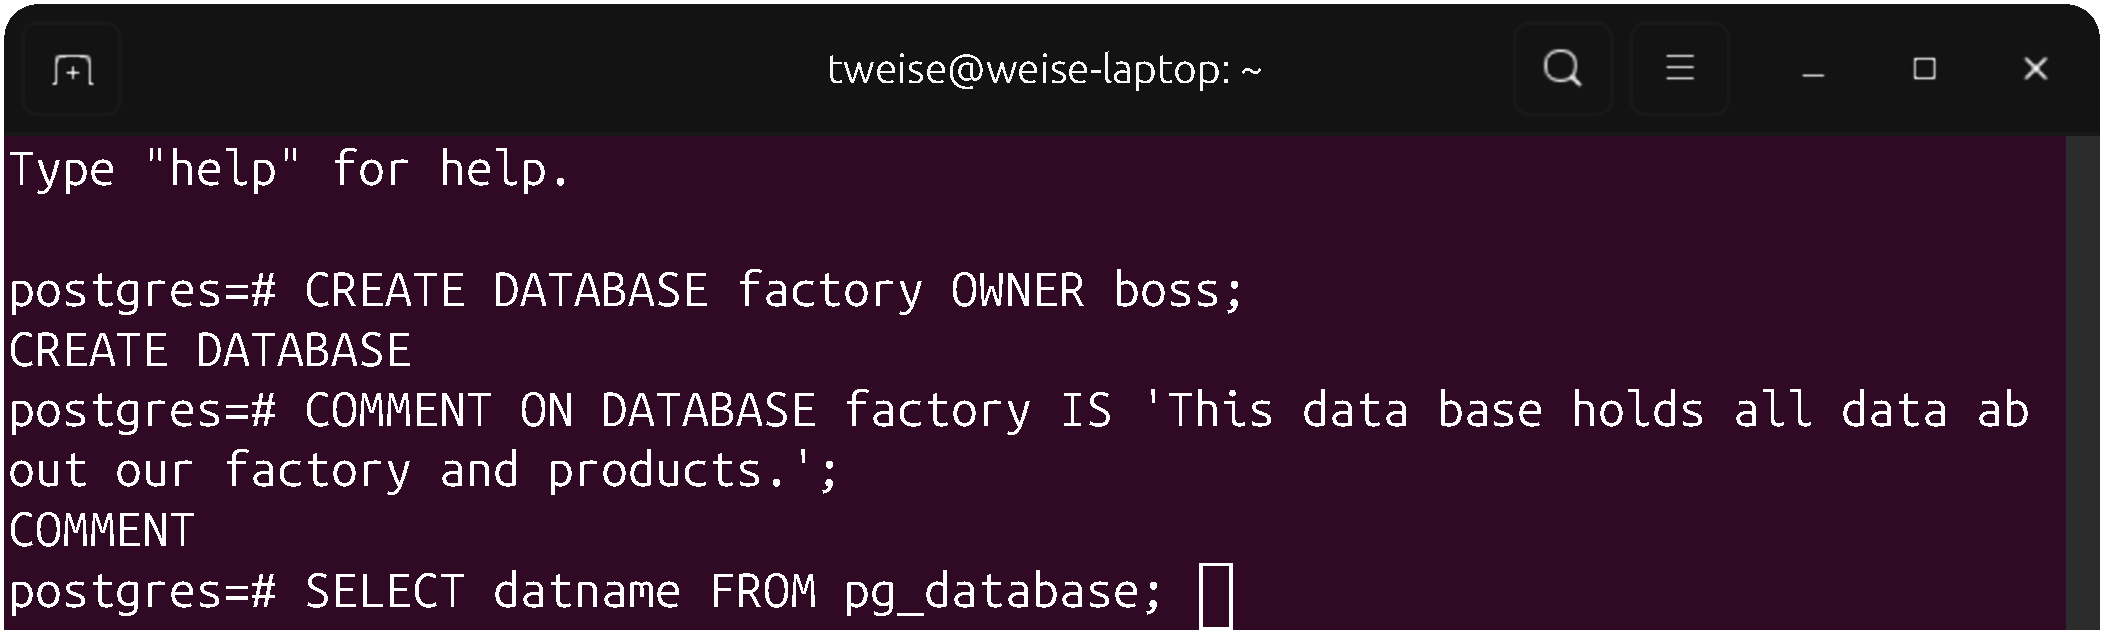
\includegraphics[width=0.67\linewidth]{\currentDir/createDB07selectDatname}}}%
%
\floatRowSep%
%
\subfloat[][%
The command will print all \pglspl{db} on the current system. %
On this installation, there are 7~\pglspl{db}, on your fresh installation, there will be fewer. %
The command may enter a paginated view, as is the case here.%
\label{fig:createDB08selected}%
]{\parbox[t]{0.99\linewidth}{\centering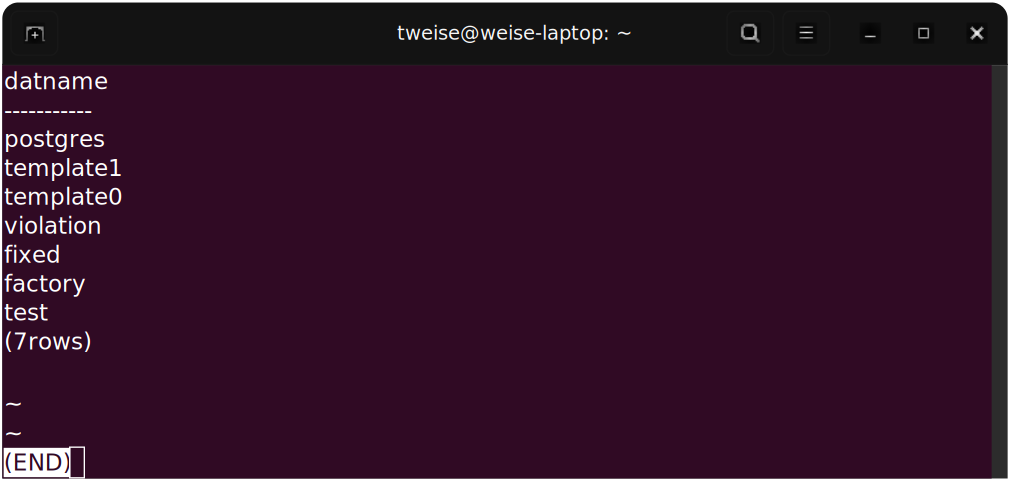
\includegraphics[width=0.67\linewidth]{\currentDir/createDB08selected}}}%
%
\caption{Creating a new \db, adding a comment to it, and checking whether it really was created, all via \psql.~(Continued)}%
\end{figure}%
%
\begin{figure}%
\centering%
\ContinuedFloat%
%
\subfloat[][%
If the paginated view was entered, you can leave it by pressing~\keys{q}. %
If it was not entered, the command will directly return.%
\label{fig:createDB09selectedQ}%
]{\parbox[t]{0.99\linewidth}{\centering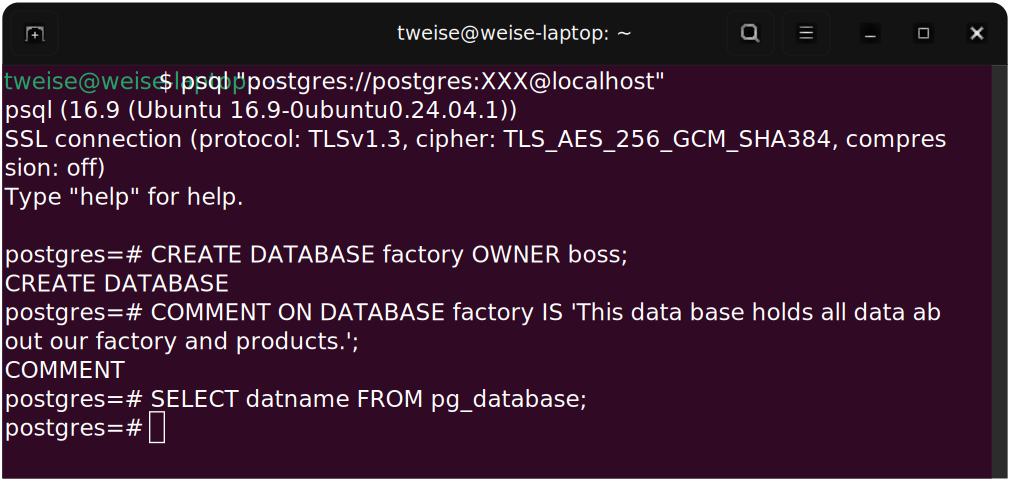
\includegraphics[width=0.67\linewidth]{\currentDir/createDB09selectedQ}}}%
%
\floatRowSep%
%
\subfloat[][%
We left the paginated result view and now want to leave this \psql\ session, by typing~\sqlil{\\q}\sqlIdx{{\textbackslash}q} and hitting~\keys{\enter}.%
\label{fig:createDB10quit}%
]{\parbox[t]{0.99\linewidth}{\centering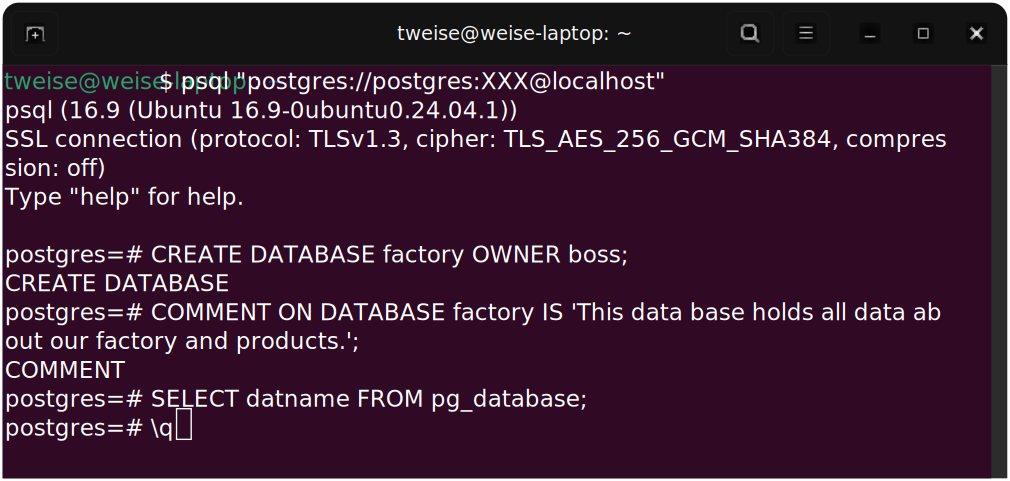
\includegraphics[width=0.67\linewidth]{\currentDir/createDB10quit}}}%
%
\floatRowSep%
%
\subfloat[][%
We are back in the normal \pgls{terminal}.%
\label{fig:createDB11done}%
]{\parbox[t]{0.99\linewidth}{\centering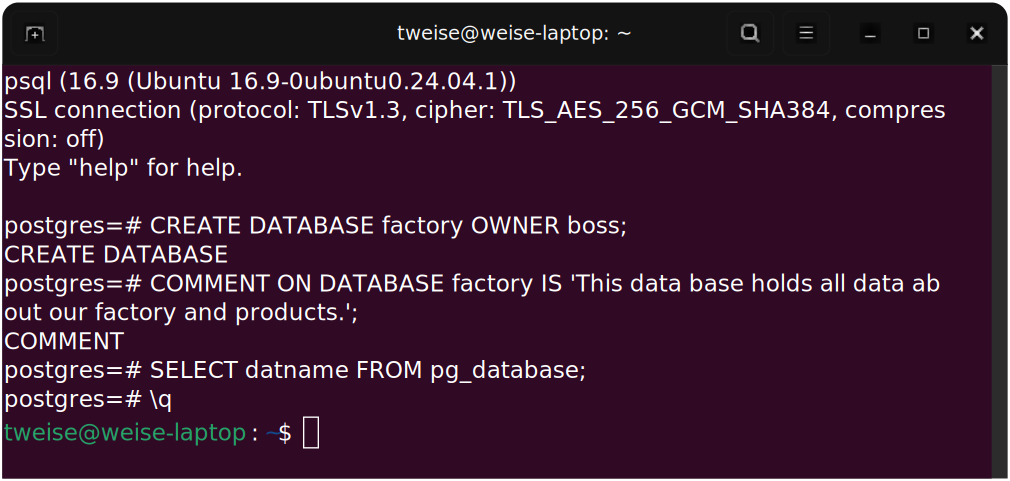
\includegraphics[width=0.67\linewidth]{\currentDir/createDB11done}}}%
%
\caption{Creating a new \db, adding a comment to it, and checking whether it really was created, all via \psql.~(Continued)}%
\end{figure}%
%
\gitLoadAndExecSQL{factory:create_database}{}{factory}{create_database.sql}{}{}{}%
\listingSQLandOutput{factory:create_database}{%
Using \sql\ to create a database for user \textil{boss}.%
}{}%
%
Having created the new user~\inQuotes{boss}, we can now create the \db\ \inQuotes{factory} to be owned and worked on by that user~\sqlil{boss}.
For this, we first open a new \psql\ session in~\cref{fig:createDB01start,fig:createDB02started}.
Notice that we still need to execute this command under the \pgls{dba} role \textil{postgres}.
Also, we can put the connection~\pgls{URI} inside of quotes~(\bashil{"..."}), which is useful if, for example, the password contains strange characters.
This user has the right to create \pglspl{db} for other users which can then work with them.
We then need to execute a single \sql-command, namely\sqlIdx{CREATE!DATABASE}\sqlIdx{DATABASE}\sqlIdx{OWNER}:
%
\sqlSyntax{syntax:create_database}{syntax/create_database.sql}%
%
Thus, all we have to do is to type the \sql\ command \sqlil{CREATE DATABASE factory OWNER boss;}\sqlIdx{CREATE!DATABASE}\sqlIdx{DATABASE}\sqlIdx{OWNER} in \cref{fig:createDB03createDatabase}.
This command pretty much explains itself.
It will create a new \db\ with the name \textil{factory}.
The user \textil{boss} will be owner of this \db, i.e., they will have full access to add and manipulate its data.
The command completes successful.
No error message appears and the command is printed back to us in \cref{fig:createDB04dbCreated}.

Documentation is a very important task in the whole field of software engineering.
It is always a good idea to store lots of comments that explain each \db, table, column, constraint, role, user, view, stored procedure, and whatever other object could exist on a \dbms.
Usually, to keep the examples small enough to fit on single pages, we will not have enough space for that.
However, here, at our very first \db, let's do it right:
In \cref{fig:createDB05comment}, we use the \sqlilIdx{COMMENT ON} command to store a comment that describes the purpose of our \db\ \sqlil{factory}.
This command also succeeds and is printed back to us in \cref{fig:createDB06commented}.%
%
\begin{sloppypar}%
We can also get a list of all the \pglspl{db} in our system.
For this purpose, we write \sqlil{SELECT datname FROM pg_database;}\sqlIdx{SELECT{\idxdots}FROM}\sqlIdx{pg\_database} in \cref{fig:createDB07selectDatname}.
See, all the names of all \pglspl{db} inside the \postgresql\ \dbms\ are stored in the column~\sqlilIdx{datname} of the table~\sqlilIdx{pg\_database}.\footnote{%
On other \pglspl{dbms}, the \pglspl{db} may be stored differently.}
If we run this command \emph{before} creating the new \db\ on a fresh \postgresql\ installation, we find that it will list some standard \pglspl{db}, which we will ignore here.%
\end{sloppypar}%
%
On the installation where I executed it, there were some more \pglspl{db}, so the command found seven \pglspl{db}.
Sometimes, if a lot of data is returned by an \sql\ command, \psql\ will change into a paginated mode, as shown in \cref{fig:createDB08selected}.
There, we can see the \pglspl{db}.
We can then exit this mode simply by pressing~\keys{q} in \cref{fig:createDB09selectedQ}.

This takes us back into our \psql\ terminal session, which we now will leave by typing in~\sqlil{\\q}\sqlIdx{{\textbackslash}q} in \cref{fig:createDB10quit}.
This ejects us back into the normal \pgls{terminal} in \cref{fig:createDB11done}.

All of the above commands are combined into a single script in \cref{lst:factory:create_database}.
\Cref{exec:factory:create_database} shows their output when being executed on a clean and fresh \postgresql\ installation~(but after the user~\sqlil{boss} was created, obviously).%
%
\FloatBarrier%
\endhsection%
%
